\documentclass[a0,final, portrait]{inriaposter}

\usepackage[utf8]{inputenc}
\usepackage[OT1]{fontenc}
\usepackage[french]{babel}
\usepackage{amsfonts, amsmath, amssymb, amsthm, dsfont, amsthm}
\usepackage{paralist}
\usepackage{wrapfig}

\usepackage{caption}
\usepackage{subcaption}

\usepackage{graphics}
\usepackage{graphicx}

\usepackage{epstopdf}

\providecommand{\mtx}[1]{\mathbf{#1}}

\begin{document}

\sffamily

\postertitle%
{Poppy 2.0: Robotique modulaire et open-source}
{Matthieu Lapeyre, Nicolas Rabault, Pierre-Yves Oudeyer}{Flowers Team,  INRIA / France}


\vfill
\Large
\begin{multicols}{2}

\blockabstract{
\textbf{Poppy 2.0 vise a créer des modules robotique tous compatible les uns avec les autre. Chacun de ces module offre une fonction dédier à la robotique. Ces module doivent être accessible quel que soit le niveau de l'utilisateur.}
}

% \block{Overview}{
% \begin{center}
%     \includegraphics[width=0.9\columnwidth]{images/poppy.png}
% \end{center}
% }

\block{Mécanique}{

Les modules poppy 2.0 doivent être en mesure de s'interfacer mécaniqueemnt de façons simple afin de permettre une intégration simple dans le plus grans nombre de cas :
    \begin{itemize}
        \item \textbf{Forme des modules :} Les modules ont la forme de cubes afin de
        multiplier les possibilité de montage.
        \item \textbf{Taille des modules :} Les modules ont des taille multiple de 12.
        \item \textbf{Compatibilité méchanique :} Les modules doivent être compatible avec des pièces imprimé en 3D ou avec des plaque découpé au laser.
    \vspace{1cm}
    \begin{center}
        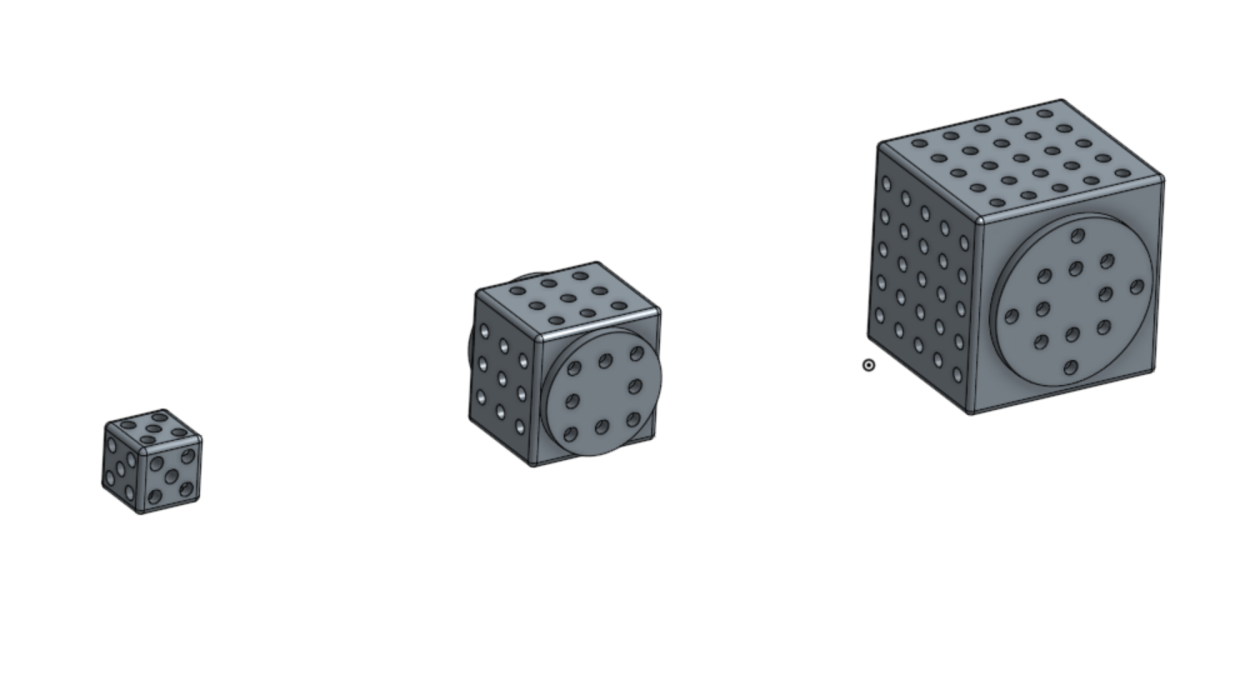
\includegraphics[width=0.9\columnwidth]{images/meca_module.png}
    \end{center}
        \item \textbf{Mécanique autogénéré :} Une appli web permettra de générer des pîèce imprimable entre les modules.
    \vspace{1cm}
    \begin{center}
        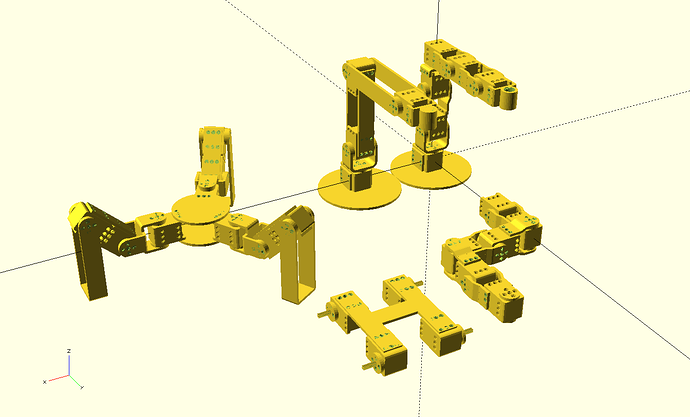
\includegraphics[width=0.9\columnwidth]{images/poppy_creatures.png}
    \end{center}
    \end{itemize}
}

\block{Electronique}{
Le montage éléctroniqe doit être le plus simple et souple possible :
    \begin{itemize}
        \item \textbf{Connectique :} La connectique est normalisé, une entré et une sortie pour chaque module.
        \item \textbf{Montage :} Les modules se branche en série les uns sur les autres. Il y aura un module HUB pour les branchement en étoile.
        \item \textbf{Identification :} Au démarage du robot chaque module se voit attribuer une adresse relative a son emplacement au démarage du robot.
    \end{itemize}
    \vspace{1cm}
    \begin{center}
        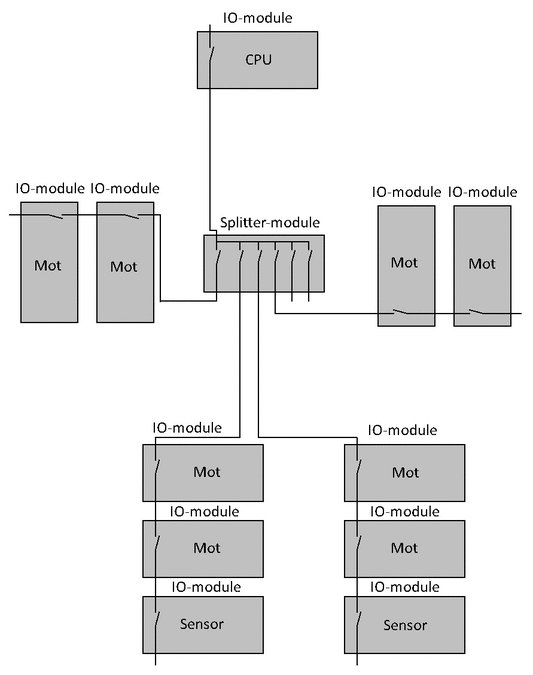
\includegraphics[width=0.5\columnwidth]{images/arch.jpg}
    \end{center}
}

\block{Structure logiciel des modules}{
% \vspace{1cm}
% \begin{center}
%     \includegraphics[width=\columnwidth]{images/poppy-explauto.png}
% \end{center}
Les modules doivent tous avoir une architecture logiciel unifier pour les rendre compatible :
\begin{itemize}
    \item \textbf{Bootloader :} La gestion de l'adressage dynamique et du démarrage sera inspiré du bootloader d'arduino afin de garder la compatibilité avec cetenvironement.
    \item \textbf{Communication :} Une librairie permettra de simplifier la communication entre les modules et sera accessible a tous les developpeurs.
    \item \textbf{Application :} Chaque module peut avoir sa propre application unique pour cela un espace de code dédier au module et au programme utilisateur sera aloué.
    \vspace{1cm}
    \begin{tabular}{cc}
        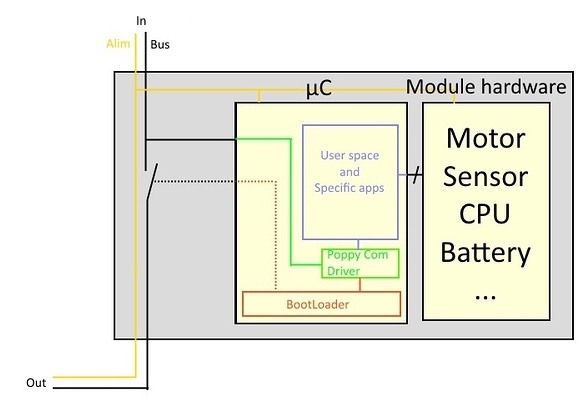
\includegraphics[width=0.45\columnwidth]{images/modul_arch.jpg} &
        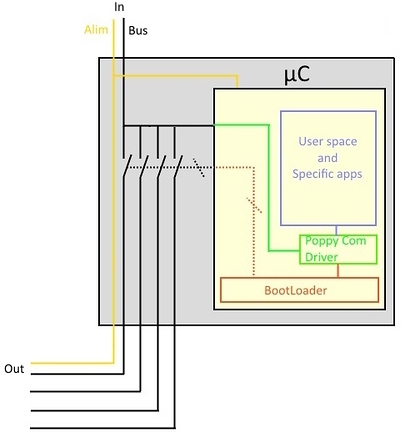
\includegraphics[width=0.45\columnwidth]{images/splitter_arch.jpg}
    \end{tabular}
\end{itemize}
}
\block{Structure logiciel haut niveau}{
% \vspace{1cm}
% \begin{center}
%     \includegraphics[width=\columnwidth]{images/poppy-explauto.png}
% \end{center}
Les modules doivent tous avoir une architecture logiciel unifié pour les rendres compatible :
\begin{itemize}
    \item \textbf{Librairie multilangage :} La librairie de controle de Poppy pourra être utiliser avec différent langage.
    \item \textbf{Programmation visuelle :} Poppy 2.0 sera compatible avec Snap.
    \vspace{1cm}
    \begin{center}
        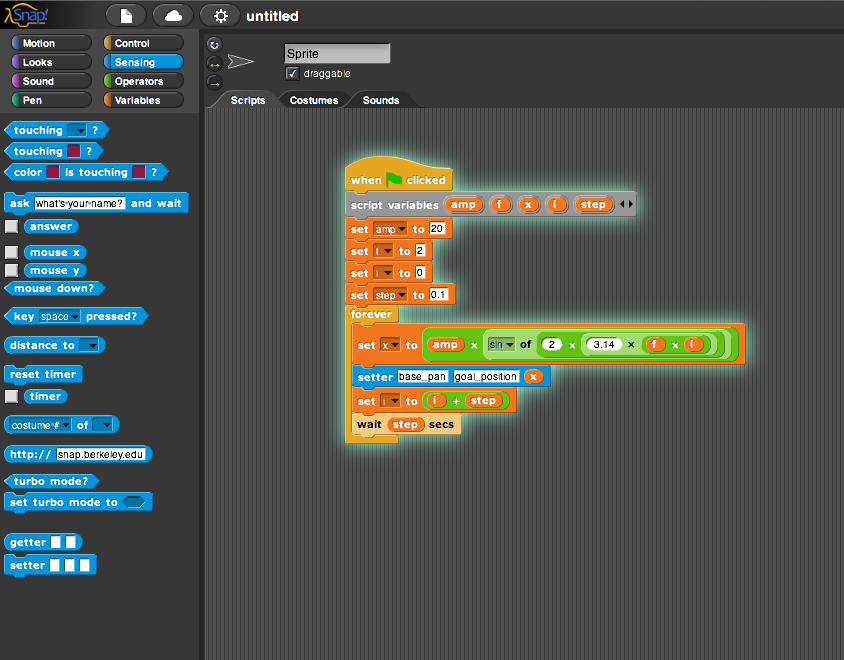
\includegraphics[width=0.4\columnwidth]{images/snap.png}
    \end{center}
    \item \textbf{Application web:} Un IDE sur le navigateur.
    \item \textbf{Compatibilité avec Poppy 1:} tous les contenu pédagogique développer pour Poppy 1 restera compatible avec l'architecture Poppy 2.0.
\end{itemize}
}
% \block{References}
% {
% 	% \vspace{-10pt}
% 	\nocite{*}
% 	\bibliographystyle{abbrv}
% 	\renewcommand{\section}[2]{}% Hack to remove bibliography title
% 	\bibliography{ref}
% 	\vspace{-10pt}
% }

\end{multicols}
\vfill
\end{document}
